\item \textbf{{[}ALVL/9597/2013/P2/Q1{]} }

A dental practice currently uses a computer system to store details
of its patients, staff and appointments in separate files.

The practice manager and the receptionist have their own computers
for accessing and updating the files.

The system produces a small number of reports.

An updated system is to be produced by a software company. The updated
system will use a database. In the updated system the dentists will
be given a hand-held device to use in their rooms for accessing and
updating the patient records. The new system will also be capable
of producing additional reports.

The software company has software engineers who have expert skills
in specific areas of software development. A number of the engineers
will be involved in the development of the updated system.
\begin{enumerate}
\item Describe and justify three methods which can be used to determine
what further reports are required from the updated computer system.
{[}6{]}
\item The work to update the system is partly managed by the following Program
Evaluation and Review Technique (PERT) chart.

A - investigation 

B - analysis 

C - design of database 

D - design of reports 

E - design of screen displays for dentists 

F - transfer of data from files into database 

G - documentation produced 

H - acceptance testing 

I - hand over to customer

Time is measured in weeks.
\begin{center}
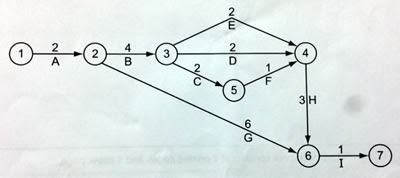
\includegraphics[width=0.5\paperwidth]{C:/Users/Admin/Desktop/Github/question_bank/LyX/static/img/9597-ALVL-2013-P2-Q1-1}
\par\end{center}
\begin{enumerate}
\item State the critical path.\hfill{} {[}1{]}
\item State the minimum time in which the updated system could be operational.
\hfill{}{[}1{]}
\item For activity E state the 
\begin{itemize}
\item earliest Start time 
\item earliest Finish time 
\item latest Start time
\item latest Finish time\hfill{}{[}4{]}
\end{itemize}
\end{enumerate}
\item {}\textcolor{white}{\_}
\begin{center}
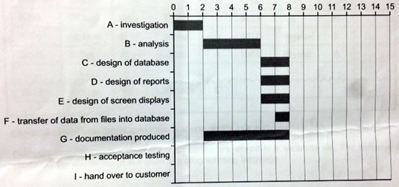
\includegraphics[width=0.5\paperwidth]{C:/Users/Admin/Desktop/Github/question_bank/LyX/static/img/9597-ALVL-2013-P2-Q1-2}
\par\end{center}

The Gantt chart above is based on the information in part \textbf{(b)}.
The timing of two activities is missing and also the timing of one
of the activities shown is incorrect.

Draw a sketch of the Gantt chart to show the correct version. \hfill{}{[}4{]}
\item Explain how the Gantt chart can help with the work that the software
engineers have to carry out. \hfill{}{[}2{]}
\item A small team is put together to consider security aspects of the updated
system.
\begin{enumerate}
\item Identify \textbf{two} possible members of the team and justify your
choice.\hfill{} {[}4{]}
\end{enumerate}
The team have to produce a report to which they all make a contribution.
The report is stored on a network. Each member of the team has access
to allow them to add their contribution.
\begin{enumerate}
\item[ii]  Give \textbf{two} examples of unethical behaviour by a team member.\hfill{}
{[}2{]}
\end{enumerate}
\item Name and describe \textbf{two} types of documentation produced for
this project.\hfill{} {[}6{]}

\noindent\fbox{\begin{minipage}[t]{1\columnwidth - 2\fboxsep - 2\fboxrule}%
End-User documentation 
\begin{itemize}
\item for actual users of system to learn about features and how to use
them 
\item minimum/recommended hardware and software system requirements (operating
system, version, processor, amount of RAM and hard disk space, etc.) 
\item installation guide + step by step guide of how to perform a task or
use a feature 
\item frequently asked questions (FAQ) for common troubleshooting problems
and solutions 
\item support contact information, safety instructions, warranty information
\end{itemize}
Technical documentation
\begin{itemize}
\item for developers to document technical requirements and features of
system
\item system objectives and scope 
\item input and output/report specifications 
\item data storage/database specification 
\item modules/processes and algorithms 
\item user interfaces and application programming interfaces (APIs) 
\item testing
\item implementation/deployment 
\item bugs report and known issues
\end{itemize}
%
\end{minipage}}
\end{enumerate}
The hand-held devices the dentists use in their practice rooms will
be networked. Both client-side scripting and server-side scripting
will be used in the new software which is produced. An intranet with
a web server will be created. Web browsers will be used on the hand-held
devices.
\begin{enumerate}
\item[(g)]  Describe three possible uses of the device.\hfill{} {[}6{]}
\item[(h)]  For each scripting method, client-side scripting and server-side
scripting, give an appropriate example. Justify your response.\hfill{}
{[}4{]}
\end{enumerate}